\section{LayerLSH: Rebuild Basic LSH}
\label{sec:reclsh}

In this section, we rebuild the basic LSH index \cite{datar,Gionis:1999:SSH:645925.671516} by exploring the density of hash values and propose LayerLSH.


\subsection{LayerLSH Structure}
\label{sec:layerlsh:overview}

As illustrated in Section \ref{sec:intro}, the query falling in dense buckets tends to result in high cost, while the query falling in sparse buckets tends to result in low accuracy. Our idea is to split the dense buckets and merge the sparse buckets, which is simple but empirically shown to be effective (Section \ref{sec:expr}). The basic LSH hashes the objects to a number of buckets in $l$ tables. With respect to each hash table, the similar objects are hashed to the same bucket with high probability. Suppose we have a set of 2-D data objects distributed as shown in the top of Figure \ref{fig:overview}. They are hashed to different buckets in two hash tables. Some of the buckets are lightly loaded, while some are heavily loaded. LayerLSH will rehash the objects residing in an overloaded bucket to a new set of hash tables, such that the overloaded bucket is rehashed into multiple groups of smaller buckets where each group corresponds to a new hash table. The overloaded buckets are rehashed recursively until no overloaded one exists. At meanwhile, the underloaded bucket will not be further processed but only be marked. When a query falls into the underloaded bucket, the query algorithm will simply expand the search scope and search the ``nearby'' buckets to improve the accuracy.

\begin{figure}[t]
\vspace{-0.1in}
    \centerline{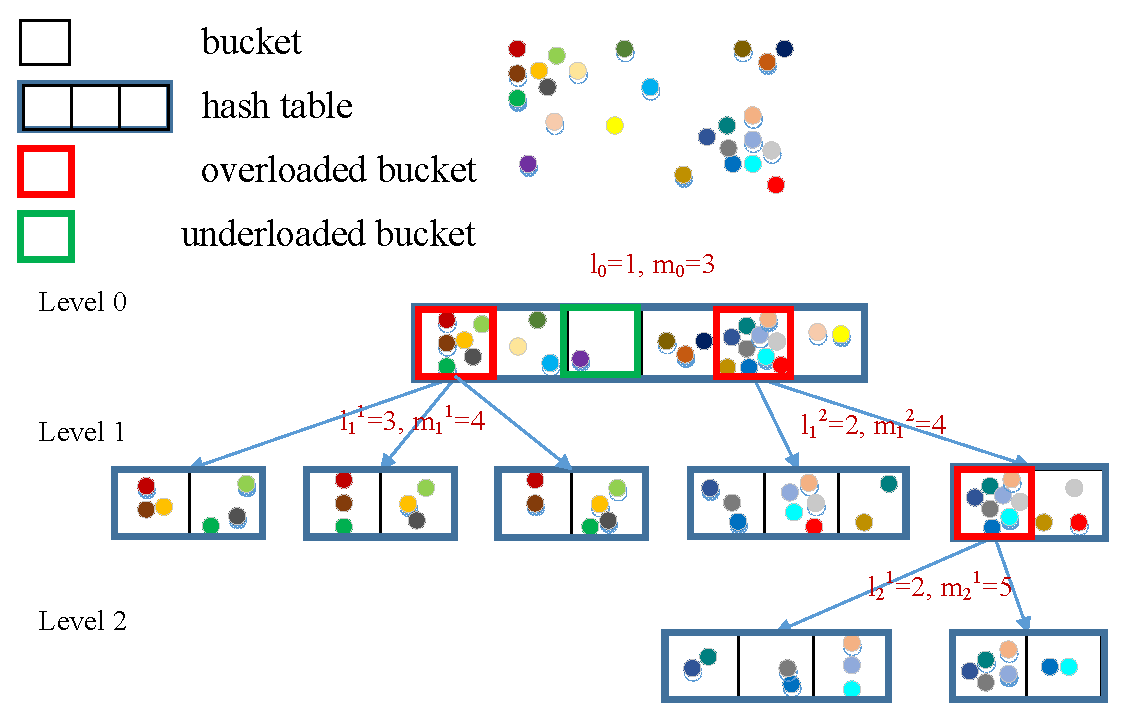
\includegraphics[width=3.2in]{fig/overview.eps}}
     \vspace{-0.05in}
    \caption{An illustrative example of LayerLSH structure (a bucket with more than 5 objects is considered as an overloaded bucket).}
    \label{fig:overview}
    \vspace{-0.2in}
\end{figure}

It is notable that since limiting bucket size will reduce the accuracy from probability theory's point of view (as shown in Equation (\ref{eq:prob})). The objects in the overloaded bucket should be copied to more than one hash tables to compensate for the reduced accuracy. This is for sustaining the expected accuracy $P$ as depicted in Equation (\ref{eq:prob2}), which will be described in detail in Section \ref{sec:layerlsh:param}. Since the overloaded buckets are rehashed recursively, multiple layers of LSH tables are constructed. The root level (level 0) of the LayerLSH is exactly the same as the original LSH. The hash tables in higher levels are the new generated LSH tables for the rehashed buckets. Figure \ref{fig:overview} shows an illustrative example of the \emph{\textbf{multi-layered}} tree-like structure.

%When an overloaded bucket is split, $l$ independent \emph{child hash tables} are created, where the split bucket is referred to as \emph{parent bucket}. The points in the parent bucket are rehashed in these child hash tables. The contents (objects) of the child tables are copies of the parent bucket, so that the objects in the split bucket have $l$ copies. Not only the level-0 bucket can be split but also the overloaded buckets at higher levels. Therefore, a \emph{\textbf{multi-layered}} tree-like structure is formed.


\subsection{Building LayerLSH}
\label{sec:layerlsh:param}

We rebuild the original hash tables in terms of two factors, the user specified expected recall and precision. Let $\text{KNN}(q,O)$ denote the set of $k$NNs of $q$. Given a query $q$ and a set of objects $O$, an approximate $k$NN query algorithm returns a set of candidates $\mathcal{C}$. We have the \textbf{recall} $\alpha=\frac{|\mathcal{C}\cap \text{KNN}(q,O)|}{|\text{KNN}(q,O)|}$, which implies the accuracy, and the \textbf{precision} $\beta=\frac{|\mathcal{C}\cap \text{KNN}(q,O)|}{|\mathcal{C}|}$, which implies the efficiency. Given $\alpha$ and $\beta$, we study the lower/upper bound size of each bucket as follows.

\begin{prop}
\label{theorem:bucketsize}
\textbf{(Bucket Size Constraints)} When using LSH with $l$ hash tables to answer $k$NN query, with an expected recall $\alpha$ and an expected precision $\beta$, the bucket size $S$ of each hash table has the following constraints:
\begin{equation}\label{eq:bucketsize}
    k\cdot(1-\sqrt[l]{1-\alpha})\leq S\leq \frac{k}{\beta\cdot l}.
\end{equation}
\end{prop}
\begin{proof}
Suppose the LSH parameters are $\{l, m, w\}$. In each of the $l$ hash table, the expected size of the bucket that $q$ falls in is $\overline S=\sum_{o\in O}p(|q,o|,w)^{m}$ where $p(s, w)^m$ is defined in Equation (\ref{eq:prob}) and (\ref{eq:prob1}). Let $s_{(q,k)}$ denote the distance from $q$ to its $k$th NN. Then we have
\begin{equation}\label{eq:recall2}
\begin{aligned}
  \overline S=\sum_{o\in O}p(|q,o|,w)^{m}&\geq \sum_{o\in \text{KNN}(q,O)}p(|q,o|,w)^{m}\\
                                        &\geq k\cdot p(s_{(q,k)},w)^m\\
                                        &\geq k\cdot(1-\sqrt[l]{1-\alpha}),
\end{aligned}
\end{equation}
The first ``$\geq$'' is true because the candidates for summation is reduced from $O$ to $\text{KNN}(q,O)$. The second ``$\geq$'' is true because for any $|q,o|\leq s_{(q,k)}$ we have $p(|q,o|,w)\geq p(s_{(q,k)},w)$ according to Equation (\ref{eq:prob}). The third ``$\geq$'' is true because in order to achieve the overall recall $\alpha$ over $l$ hash tables, the probability that $q$ and any of its $k$NNs collide in a specific hash table should be no less than $1-\sqrt[l]{1-\alpha}$ according to Equation (\ref{eq:prob2}). If we can make $p(s_{(q,k)},w)^m\geq 1-\sqrt[l]{1-\alpha}$ for $q$'s $k$th NN, it is also true for any other $k$NNs. Thus, the bucket size $S$ should satisfy $S\geq k\cdot(1-\sqrt[l]{1-\alpha})$.

When all of $q$'s $k$NNs are contained in the returned candidates set, i.e., $\text{KNN}(q,O)\subset\mathcal{C}$, $|\mathcal{C}|$ can be as large as $\frac{k}{\beta}$ to satisfy the expected precision, otherwise $|\mathcal{C}|$ has to be smaller. Thus, $\frac{k}{\beta}$ is the upper bound of $|\mathcal{C}|$. Since there are $l$ hash tables, the candidates are retrieved from $l$ buckets. Let us assume the candidates are collected evenly from $l$ hash tables. Thus, the bucket size $S$ should satisfy $S\leq \frac{k}{\beta\cdot l}$.
\end{proof}

Note that, satisfying the above constraints does not necessarily guarantee the expected recall and precision but helps us identify the underloaded and overloaded buckets.

Given the constraints of the bucket size, we propose Algorithm \ref{alg:split} to recursively rehash the overloaded buckets to build LayerLSH index. The input includes the original LSH tables (i.e., level-0 hash tables), the LSH parameters set $\{l,m,w\}$, the number of returned NNs $k$, the expected recall $R=\alpha$, and the expected precision $P=\beta$. With respect to each hash table, the recall is relaxed to $R'=1-\sqrt[l]{1-R}$, and the precision is tightened to $P'=P\cdot l$ (Line 2). Then, we have the lower bound size ($T_l=k\cdot R'$) and upper bound size ($T_u=\frac{k}{P'}$) for each bucket (Line 3). We check the size of each bucket of each hash table. For the overloaded bucket that contains more than $T_u$ objects (Line 7), we first determine a new set of child LSH parameters (Line 8), based on which the objects in that bucket are rehashed into a new set of hash tables (Line 9). The overloaded buckets are rehashed by recursively invoking this process until no bucket is overloaded (Line 10). For the underloaded bucket that contains fewer than $\frac{k\cdot\alpha}{l}$ objects (Line 11), we mark it for future use in query processing (Line 12).

\SetAlFnt{\small\sffamily}
\SetInd{0.55em}{0.5em}
\setlength{\textfloatsep}{0pt}
\begin{algorithm}[t]
\SetNoFillComment
\SetKwProg{Fn}{Function}{:}{end}
\SetKwFunction{RecSplit}{RecursSplit}\SetKwFunction{FindLSHParam}{FindParam}\SetKwFunction{LSH}{LSH}
\SetKwInOut{Input}{input}\SetKwInOut{Output}{output}

\Input{LSH hash tables $HT=\{HT_1,\ldots,HT_l\}$, LSH parameters $\{l,m,w\}$, $k$, $R=\alpha$, $P=\beta$}
\Output{LayerLSH hash tables set}
\BlankLine
\Fn{\RecSplit{$HT$, $\{l,m,w\}$, $R$, $P$}}{\
    $R'=1-\sqrt[l]{1-R}$, $P'=P\cdot l$\;
    $T_l=k\cdot R'$, $T_u=\frac{k}{P'}$\;
    \ForEach{$HT_i$ in $HT$}{
        \ForEach{bucket $b$ in $HT_i$}{
            $S\leftarrow$ size of $b$\;
            \If{$S>T_u$}{
                $\{l_c,m_c,w_c\}\leftarrow$\FindLSHParam($\{l,m,w\}$, $S$, $P'$)\;
                $HT_{child}\leftarrow$\LSH($b$, $\{l_c,m_c,w_c\}$)\;
                \RecSplit{$HT_{child}$, $\{l_c,m_c,w_c\}$, $R'$, $P'$};
            }
            \If{$S<T_l$}{
                mark $b$ as underloaded;
            }
        }
    }
}
\caption{Building LayerLSH}
\label{alg:split}
\end{algorithm}

In Algorithm \ref{alg:split}, we refer to the to-be-rehashed bucket as \emph{parent bucket} and the new LSH for this bucket as \emph{child LSH}. The core of bucket rehashing is to choose a proper new set of child LSH parameters, such that the bucket size is reduced (for efficiency) but at the same time the probability that a query and its $k$NNs collide in the same bucket is not reduced (for accuracy). We fix the LSH width parameter $w$ (We will explain the reason later). Let $\{l_p,m_p,w\}$ denote the set of parent LSH parameters, and $\{l_c,m_c,w\}$ denote the set of child LSH parameters. We use the following propositions to guide the selection of child LSH parameters.

\begin{prop}
\label{prop:accuracy}
\textbf{(For Accuracy)} Let $s_{(q,k)}$ denote the distance from a query $q$ to its $k$th NN. Suppose we can find a $r^*$ such that $r^*\geq s_{(q,k)}$ for any $q$. In order to NOT reduce the expected recall, the child LSH parameters $\{l_c,m_c\}$ should be chosen to satisfy:
\begin{equation}\label{eq:sustainprob}
    1-(1-p^{m_p+m_{c}})^{l_{c}}=p^{m_{p}},
\end{equation}
where $p=p(r^*,w)$ is defined in Equation (\ref{eq:prob}).
\end{prop}
\begin{proof}
Since $\forall q, r^*\geq s_{(q,k)}$, we have $p(r^*,w)^{m_p}\leq p(s_{(q,k)},w)^{m_p}$. That is, the probability that any query $q$ and its $k$th NN collide in the same bucket is no less than $p(r^*,w)^{m_p}$. If the probability $p(r^*,w)^{m_p}$ could be sustained after bucket rehashing, the probability that $q$ and any of its $k$NNs fall in the same bucket will not reduce, so that the expected recall $\alpha$ is guaranteed. Accordingly, in terms of Equation (\ref{eq:prob2}), the child LSH parameters $\{l_c,m_c,w\}$ should be chosen such that $1-[1-p(r^*,w)^{m_p+m_{c}}]^{l_{c}}\geq p(r^*,w)^{m_{p}}$. Further, since all the objects in child hash tables are originated from the parent bucket, the collision probability in child hash tables will never be greater than $p(r^*,w)^{m_{p}}$. Therefore, we aim to make $1-[1-p(r^*,w)^{m_p+m_{c}}]^{l_{c}}=p(r^*,w)^{m_{p}}$.
\end{proof}

In practice, $r^*$ can be approximately estimated by sampling. A number of sample objects are randomly selected to calculate their exact $k$NNs. The median of their $k$th NNs' distances is used to estimate $r^*$.

\begin{prop}
\label{prop:efficiency}
\textbf{(For Efficiency)} Let $S$ denote the size of the overloaded bucket that $q$ falls in. In order to approximately satisfy the precision constraint, the child LSH parameter $m_c$ and $l_c$ should be chosen as follows:
\begin{equation}\label{eq:forefficiency}
\begin{aligned}
    m_c&=\Big\lceil log_{p}\Big(\frac{k}{S\cdot\beta\cdot l_p}\Big)\Big\rceil,\\
    l_c&\leq\Big\lfloor\frac{k}{S_c^*\cdot\beta\cdot l_p}\Big\rfloor,
\end{aligned}
\end{equation}
where $p=p(r^*,w)$ is defined in Equation (\ref{eq:prob}), $\beta$ is the expected precision, and $S_c^*$ is the biggest bucket size among all child hash tables.
%Assume $S$ is approximately proportional to $X_{r^*}\cdot p(r^*,w)^m_{p}$, where $X_{r^*}$ is the exact number of objects whose distances to $q$ are less than $r^*$, i.e., $S\approx \gamma\cdot X_{r^*}\cdot p(r^*,w)^m_{p}$.
\end{prop}
\begin{proof}
The expected size of the bucket that $q$ falls in is $\overline S=\sum_{o\in O}p(|q,o|,w)^{m_p}$. From this equation, we learn that the actual bucket size relates to two factors, 1) the number of ``close'' objects to $q$ and 2) the probability that these ``close'' objects fall in $q$'s bucket (determined by $\{m_p,w\}$). The more ``close'' objects to $q$, the more likely $S$ is larger. The larger $m_p$ is, the more likely $S$ is smaller. Let $X=\{o:|q,o|\leq r^*\}$ denote the set of objects within a range of $r^*$, which are considered as ``close'' objects. In other words, $|X|$ implies $q$'s density. Then we assume that the bucket size $S$ is proportional to $|X|$, i.e., $S\propto |X|$. On the other hand, to simplify the analysis and obtain an approximate answer, we assume that the probability for all objects in $X$ falling in $q$'s bucket is proportional to $p(r^*,w)^{m_p}$ that is fixed for all objects in $X$, i.e., $S\propto p^{m_p}$ where $p=p(r^*,w)$. Thus, we have $S\propto|X|\cdot p^{m_p}$.

In order to satisfy the efficiency constraint $\frac{k}{S\cdot l_p}\geq\beta$, the bucket size $S$ should be reduced to less than $\frac{k}{\beta\cdot l_p}$. Since $S\propto|X|\cdot p^{m_p}$, $|X|\cdot p^{m_p}$ should be correspondingly reduced to $|X|\cdot p^{m_p+m_c}$. Therefore, we should choose $m_c$ to satisfy the following equation:
\begin{equation}\label{eq:forefficiency2}
    \frac{S}{\frac{k}{\beta\cdot l_p}}=\frac{|X|\cdot p^{m_p}}{|X|\cdot p^{m_p+m_c}}.
\end{equation}
Since $m_c$ should be an integer, we choose the result of the ceiling function, i.e., $m_c=\big\lceil log_{p}\big(\frac{k}{S\cdot\beta\cdot l_p}\big)\big\rceil$ to sustain the inequality of precision constraint.

On the other hand, after rehashing we also need to limit the number of child hash tables in order to satisfy the efficiency constraint. Suppose $S_{(q,i)}$ is the size of a query $q$'s bucket (or multiple child buckets if it points to child hash tables) in child hash table $i$, we need to make sure $\sum_{i=1}^{l_c}S_{(q,i)}\leq \frac{k}{\beta\cdot l_p}$. Further, suppose $S_c^*$ is the biggest bucket size among all child hash tables, we have $\sum_{i=1}^{l_c}S_{(q,i)}\leq l_c*S_c^*$. Thus, by making $l_c*S_c^*\leq\frac{k}{\beta\cdot l_p}$, i.e., $l_c\leq\big\lfloor\frac{k}{S_c^*\cdot\beta\cdot l_p}\big\rfloor$ (since $l_c$ should be an integer), we can satisfy the efficiency requirement.
\end{proof}

%Note that, $S_c^*$ is unknown before bucket rehashing. We will try a $l_c$ and rehash the bucket. If some buckets are still overloaded, the bucket rehashing process is invoked again. This is the reason why a recursive rehashing process is designed.

By combining Proposition \ref{prop:accuracy} and Proposition \ref{prop:efficiency}, we intend to obtain the available child LSH parameters $m_c$ and $l_c$, which are used during bucket rehashing (Line 8 in Algorithm \ref{alg:split}). However, there probably is no solution since the recall and precision requirements cannot be satisfied at the same time (i.e., $l_c$'s lower bound is greater than its upper bound). Furthermore, $S_c^*$ in Equation (\ref{eq:forefficiency}) is even unknown before bucket rehashing. In such a case, we first choose $m_c$ according to Equation (\ref{eq:forefficiency}), ignore the upper bound of $l_c$, and generate enough more child hash tables to sustain accuracy constraint according to Equation (\ref{eq:sustainprob}). We will further satisfy the efficiency constraint during the query processing.

The reason why we perform the analysis by fixing $w$ is explained as follows. Given a query $q$, for any point, its probability (shown in Equation \ref{eq:prob}) to collide with $q$ depends on its distance to $q$ (i.e., $s$) and the partition width $w$. If adjusting $w$ is allowed, regarding a particular point, its probability to collide with $q$ would change after rehashing. The new probability $p(s, w)$ depends on a variable $s$ since $s$ is variant for different points. That means, the analysis in Proposition \ref{prop:accuracy} or \ref{prop:efficiency} should also consider $s$, the distance from a point to a query. Obviously, $s$ is unknown in prior since query is unknown in prior. This will bring significant challenges in analyzing accuracy and efficiency. Therefore, we propose to rehash data by fixing $w$.

%Specifically, we choose $m_c$ according to Equation (\ref{eq:forefficiency}). Thus, we will obtain $l_c$'s upper bound $\big\lfloor\frac{k}{S_c^*\cdot\beta\cdot l_p}\big\rfloor$ from Equation (\ref{eq:forefficiency}) and lower bound $\big\lceil log_{(1-p^{m_p+m_c})}(1-p^{m_p})\big\rceil$ from Equation (\ref{eq:sustainprob}). However, there probably is no solution since the recall and precision requirements cannot be satisfied at the same time (i.e., $l_c$'s lower bound is greater than its upper bound). In such a case, we ignore the upper bound of $l_c$ and generate enough more child hash tables to sustain accuracy constraint. We will further satisfy the efficiency constraint during the query processing.


\begin{comment}
\begin{equation}\label{eq:meanlc}
    \overline{l_c}=\Big\lceil\frac{\frac{k}{S_c^*\cdot\beta\cdot l_p}+log_{1-p^{m_p+m_c}}(1-p^{m_p})}{2}\Big\rceil
\end{equation}
\end{comment}

\begin{comment}
\begin{prop}
\label{prop:childparam}
\textbf{(Bucket Split-Child LSH Parameters)} In order to sustain the accuracy and efficiency, the bucket split should choose child LSH parameters as follows:
\begin{equation}\label{eq:sustainprob}
\begin{aligned}
    m_c&=m_p+\Big\lceil log_{p}\Big(\frac{k}{S\cdot\beta\cdot l_c}\Big)\Big\rceil,\\
    l_c&=\lceil log_{(1-p^{m_c})}{(1-p^{m_p})}\rceil,
\end{aligned}
\end{equation}
where $p=p(r^*,w)$. $w$ is consistent with parent LSH parameter.
\end{prop}
\end{comment}


\subsection{Query Processing}
\label{sec:layerlsh:query}

There are two kinds of buckets in LayerLSH, which should be differentiated during query processing. One kind that contains similar data objects, which are referred to as \emph{data buckets}. Another kind contains the pointers to child hash tables, which are referred to as \emph{pointer buckets}. In other words, in the LayerLSH tree-like structure, the leaf nodes are data buckets, while the internal nodes are pointer buckets.

\begin{algorithm}[t]
\SetNoFillComment
\SetKwProg{Fn}{Function}{:}{end}
\SetKwFunction{LayerLSHQuery}{LayerLSHQuery}
\SetKwInOut{Input}{input}\SetKwInOut{Output}{output}

\Input{query $q$, LayerLSH tables $HT=\{HT_1,\ldots,HT_l\}$, $k$, $R=\alpha$, $P=\beta$}
\Output{$k$NN candidates set $\mathcal{C}$}
\BlankLine
\Fn{\LayerLSHQuery($q$, $HT$, $R$, $P$, $\mathcal{C}$)}{\
    $\{l,m,w\}\leftarrow$ load LSH parameters for $HT$\;
    $R'=1-\sqrt[l]{1-R}$, $P'=P\cdot l$\;
    $T_l=k\cdot R'$, $T_u=\frac{k}{P'}$\;
    \ForEach{$HT_i$ in $HT$}{
        $b\leftarrow$ locate bucket with hash key $\{h_1(q),\ldots,h_m(q)\}$\;
        \If{$b$ is a pointer bucket}{
            $HT_{child}\leftarrow$ locate the child hash tables $b$ points to\;
            \LayerLSHQuery($q$, $HT_{child}$, $R'$, $P'$, $\mathcal{C}$);
        }
        \ElseIf{$b$ is a data bucket}{
            \If{$b$ is underloaded}{
                $B\leftarrow b$\;
                \While{$|B|<T_{l}$}{
                    $b'$ find ``nearby'' bucket from $b$\;
                    $B\leftarrow B\cup b'$;
                }
                $\mathcal{C}\leftarrow\mathcal{C}\cup B$;
            }
            \Else{
                \lIf{$R$ is primary}{$\mathcal{C}\leftarrow\mathcal{C}\cup b$}
                \lElseIf{$P$ is primary}{$\mathcal{C}\leftarrow\mathcal{C}\cup b'$ s.t. $|b'|\leq T_{u}$}
                \lElse{$\mathcal{C}\leftarrow\mathcal{C}\cup b'$ s.t. $|b'|\leq\frac{T_u+\frac{\sum_{i}^{l}|b_{(q,i)}|}{l}}{2}$}
            }
        }
    }
}
\caption{Query Processing in LayerLSH}
\label{alg:lshquery}
\end{algorithm}

To answer a $k$NN query, we use Algorithm \ref{alg:lshquery} to retrieve the candidates set from multi-layered hash tables. We first read the LayerLSH parameters $\{l,m,w\}$ from the input LayerLSH tables (Line 2). With respect to each hash table, the recall is relaxed to $R'$, and the precision is tightened to $P'$ (Line 3). Then, we have the lower bound size ($T_l=k\cdot R'$) and upper bound size ($T_u=\frac{k}{P'}$) for each bucket (Line 4). Given a query $q$, we first compute its compound hash keys and project $q$ to the bucket in a particular hash table (Line 6). If the positioned bucket is a pointer bucket, the query $q$ is rehashed in multiple child hash tables along with the bucket-based $R'$ and $P'$ (Line 8), and the query algorithm is invoked recursively (Line 9).


If the positioned bucket is a data bucket and this bucket is underloaded (Line 11), we will expand the search scope and search the ``nearby'' buckets whose compound hash keys are slightly different. This searching scope is expanded to more and more buckets as soon as enough objects ($T_l$) are returned (Line 12-16). The idea of merging ``nearby'' sparse buckets is similar to multi-probe LSH \cite{mplsh}. Given the property of LSH, if an object is close to a query $q$ but not hashed to the same bucket, it is likely to be in a bucket that is ``close by'' (i.e., the hash keys of the two buckets only differ slightly). LayerLSH also designates the ``close by'' buckets by applying a \emph{hash perturbation vector} $\Delta=\{\delta_1,\delta_2,\ldots,\delta_m\}$ (e.g., $\{+1,0,\ldots,0\}$ or $\{0,-1,\ldots,0\}$) on the original compound hash key $G(q)=\{h_1(q),h_2(q),\ldots,h_m(q)\}$ and obtains the nearby bucket $G(q)+\Delta$.

%However, multi-probe LSH performs nearby bucket searching without discrimination. The search of the dense bucket and its nearby buckets will return a large number of candidates but only with a limited accuracy improvement. In contrast, LayerLSH only searches for nearby buckets for sparse queries, which is more cost efficient.


If the data bucket is not underloaded, the objects in that bucket are conditionally put into the candidates set $\mathcal{C}$ (Line 17). Recall that, it is possible that the specified recall and precision are conflict with each other. It is required to return all candidates from all hash tables in order to satisfy the recall requirement, but also required to return at most $T_u$ candidates from only a few hash tables to satisfy the precision requirement. LayerLSH will let users specify one primary choice, the expected recall $\alpha$ or the expected precision $\beta$. Then the query processing algorithm will correspondingly include all the objects in bucket to satisfy recall requirement (Line 18) or limit the number of returned candidates to satisfy precision requirement (Line 19). If both or none of recall and precision is primarily selected, LayerLSH balances these two factors and return at most $\frac{T_u+\frac{\sum_{i}^{l}|b_{(q,i)}|}{l}}{2}$ candidates, where $T_u$ is for precision requirement and $\frac{\sum_{i}^{l}|b_{(q,i)}|}{l}$ is for recall requirement (where $b_{(q,i)}$ is $q$'s bucket in the $i$th child hash table).




\begin{comment}
\begin{figure}[htb]
    \centerline{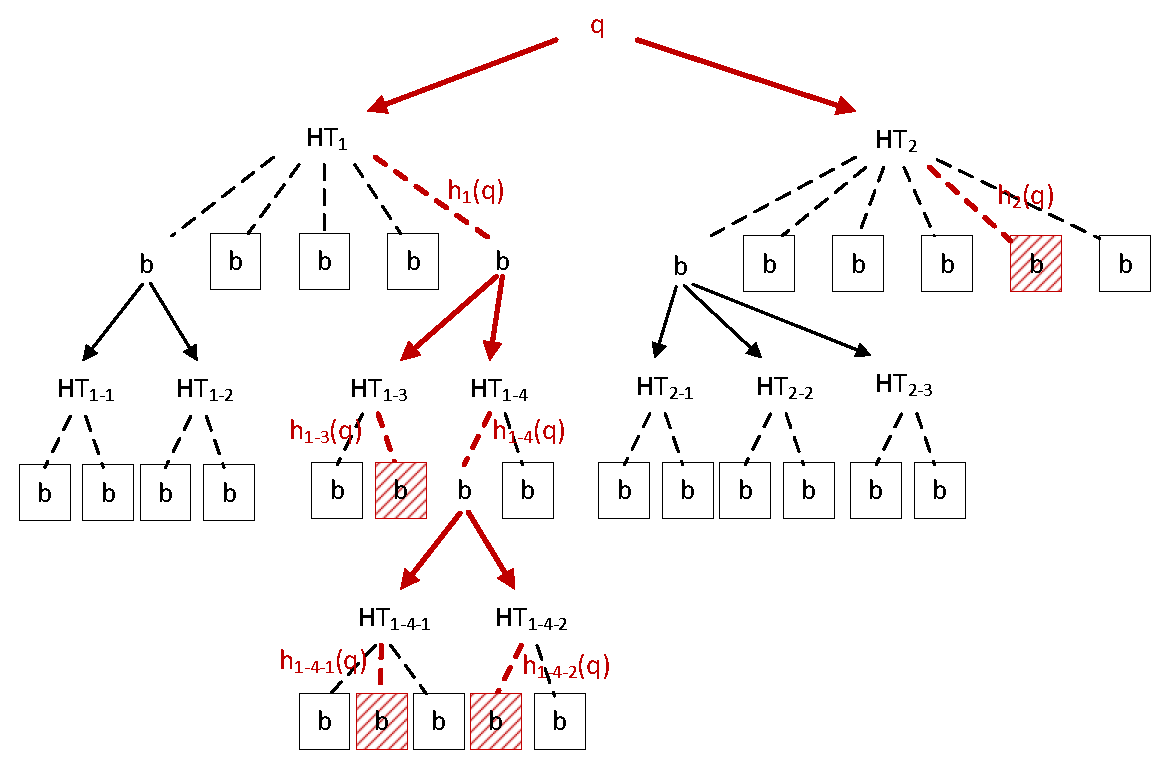
\includegraphics[width=3.2in]{fig/layerlshquery.eps}}
    \caption{Approximate $k$NN query in LayerLSH. HT denotes a hash table, and b denotes a bucket. The red lines or dashed lines show the query paths. The shadowed boxes are the data buckets which the query $q$ falls in.}
    \label{fig:layerlshquery}
\end{figure}
\end{comment}




It is noticeable that the query might expand to more and more buckets as it goes deeper in the LayerLSH tree. However, the large number of checked buckets does not necessarily lead to large number of candidates since the checked buckets are much smaller. With regard to the dense buckets, LayerLSH narrows the search scope, as a result the search is more efficient. Rather than using a large number of hash tables to achieve high search quality, we can achieve the same search quality with a smaller number of level-0 hash tables. More hash tables are only created for the dense buckets. The hashing is more targeted in terms of data distribution.

\begin{comment}
\subsection{Integrating Multi-Probe LSH}

The idea of multi-probe LSH \cite{mplsh} is simple but effective. Given the property of LSH, if an object is close to a query $q$ but not hashed to the same bucket as $q$, it is likely to be in a bucket that is ``close by'' (i.e., the hash values of the two buckets only differ slightly). Multi-probe LSH designates the ``close by'' buckets by applying a \emph{hash perturbation vector} $\Delta=\{\delta_1,\delta_2,\ldots,\delta_m\}$ on the original compound hash key $G(q)=\{h_1(q),h_2(q),\ldots,h_m(q)\}$ and obtains the nearby bucket $G(q)+\Delta$. Since similar objects should hash to the same or adjacent values (i.e., differ by at most 1), the original paper \cite{mplsh} suggests to only focus on perturbation vectors $\Delta$ with $\delta_i\in\{-1,0,1\}$.

%An $n$-step perturbation vector $\Delta$ has exactly $n$ coordinates that are non-zero. Intuitively, buckets that are returned by 1-step probing are more likely to contain objects that are close to the query object than buckets returned by 2-step probing. Therefore, the \emph{step-wise probing} first probes all the 1-step buckets, then all the 2-step buckets, and so on.

%The idea of multi-probe LSH is to expand the search scope of the relatively sparse bucket.
As illustrated in Section \ref{sec:intro}, queries that are projected to the bucket with low density suffers from the low accuracy problem. Increasing the number of hash tables would improve the search quality at the expense of more searching cost. In contrast, multi-probe LSH improves the search quality by searching nearby buckets. However, multi-probe LSH performs nearby bucket searching without discrimination. The search of the dense bucket and its nearby buckets will lead to high distance computation cost but only with a limited improvement.

LayerLSH integrates the idea of multi-probe LSH, which identifies the densities of buckets and performs more targeted nearby bucket search. That is, we only search for nearby buckets for sparse queries. Note that, there are multiple layers of buckets in LayerLSH. Since the nearby buckets are more similar at lower levels than at higher levels, when handling a sparse query the lower-level nearby buckets are given higher priority than the higher-level nearby buckets. The bucket search terminates until a predefined number of points is searched.

%the number of checked points is larger than $T$ where $T$ is the bucket limit in bucket split.


%Note that, multi-probe LSH is a probing optimization technique on the basic LSH index structure instead of a new indexing scheme. We will use it to optimize our query process in the paper.

%The original paper shows that most $k$ nearest neighbors are retrieved by only probing 1-step buckets and 2-step buckets.
\end{comment}


\subsection{Supporting Dynamic Data Stream}

To deal with dynamic data, we need to make LayerLSH support point insertions and deletions. Algorithm \ref{alg:split} can be slightly changed for updating the index structure, where the input is the continuous insertions or deletions. A point is inserted into or deleted from a specified bucket followed by checking the bucket size. If the bucket size is bigger than $T_u$ after insertions, the bucket will be split. If the bucket size is smaller than $T_l$ after deletions, it will be marked as underloaded, and several similar underloaded buckets will be searched together when query processing.  

However, the naive implementation may result in too many unnecessary bucket splits. For instance, an insertion followed by multiple deletions to a full bucket results in unnecessary bucket split. To alleviate this problem, we introduce the \textit{time window} concept and buffer these insertion/deletion operations. Basically, in a time window, if the bucket size is not larger than a \textit{maximum tolerance}, it will not be split, otherwise, it will still be split. The maximum tolerance of bucket size should be a little bit larger than $T_u$, which implies the effect of buffering. After each time window, all the buckets are evaluated to determine whether they should be split by considering the original upper bound size $T_u$. By introducing the time window based buffering, a large amount of unnecessary bucket splits can be avoided and the processing throughput can be increased, at the expanse that the query cost can be increased due to the delayed bucket split operations. The tradeoff between processing throughput and query cost can be adjusted by tuning the maximum tolerance parameter, the effect of which will be shown in Section \ref{sec:expr}.

\subsection{Index Maintenance}

In addition, LayerLSH can be implemented as a disk-based index for maintaining large data sets. Since the basic structure in LayerLSH is tree-like, it is straightforward to store the index using a tree structure. The internal nodes storing the child LSH parameters as well as the pointers to child buckets are maintained in an \emph{index file}, and the leaf nodes storing the data points are maintained in a \emph{data file}. Note that, one leaf node that stores a large bucket is written to multiple file blocks, and multiple leaf nodes storing multiple small buckets are written to a single file block to save space. Similar buckets are stored continuously in a file block to support ``nearby'' bucket search.

When answering queries, the internal nodes maintained in index file are loaded into memory for fast access, or part of them for large index. After the data buckets are positioned, the file blocks storing the candidate buckets are loaded into memory for distance measurements, followed by returning the approximate $k$NNs. To support insertion of a point, we first locate the file blocks that store the hashed buckets and then append the point data. Note that, request of a new file block might be needed if the returned file block is full. To support deletion of a point, we first locate the file blocks and label this point indicating its invalidation. A periodical recycling process is executed offline to recycle the file blocks where no valid data is contained.

\subsection{Complexity Analysis}











